\documentclass[a4paper,11pt]{exam}
%\printanswers % pour imprimer les réponses (corrigé)
 \noprintanswers % Pour ne pas imprimer les réponses (énoncé)
\addpoints % Pour compter les points
% \noaddpoints % pour ne pas compter les points
%\qformat{\textbf{\thequestion ) } }
\qformat{\textbf{Question\ \thequestion}\quad(\thepoints)\hfill} % Pour définir le style des questions (facultatif)
\usepackage{color} % définit une nouvelle couleur
\shadedsolutions % définit le style des réponses
% \framedsolutions % définit le style des réponses
\definecolor{SolutionColor}{rgb}{0.8,0.9,1} % bleu ciel
\renewcommand{\solutiontitle}{\noindent\textbf{Solution:}\par\noindent} % Définit le titre des solutions




\makeatletter

\def\maketitle{{\centering%
	\par{\huge\textbf{\@title}}%
	\par{\@date}%
	\par}}

\renewcommand{\thesection}{Exercice \arabic{section} }

\renewcommand{\thesubsection}{Partie \Alph{subsection}}   



\makeatother

\lhead{NOM Pr\'enom :}
%\rhead{\textbf{Les r\'eponses doivent \^etre justifi\'ees et r\'edig\'ees}}
\cfoot{\thepage / \pageref{LastPage}}


%\usepackage{../../pas-math}
%\usepackage{../../moncours}


%\usepackage{pas-cours}
%-------------------------------------------------------------------------------
%          -Packages nécessaires pour écrire en Français et en UTF8-
%-------------------------------------------------------------------------------
\usepackage[utf8]{inputenc}
\usepackage[frenchb]{babel}
\usepackage[T1]{fontenc}
\usepackage{lmodern}
\usepackage{textcomp}



%-------------------------------------------------------------------------------

%-------------------------------------------------------------------------------
%                          -Outils de mise en forme-
%-------------------------------------------------------------------------------
\usepackage{hyperref}
\hypersetup{pdfstartview=XYZ}
%\usepackage{enumerate}
\usepackage{graphicx}
\usepackage{multicol}
\usepackage{tabularx}
\usepackage{multirow}


\usepackage{anysize} %%pour pouvoir mettre les marges qu'on veut
%\marginsize{2.5cm}{2.5cm}{2.5cm}{2.5cm}

\usepackage{indentfirst} %%pour que les premier paragraphes soient aussi indentés
\usepackage{verbatim}
\usepackage{enumitem}
\usepackage[usenames,dvipsnames,svgnames,table]{xcolor}

\usepackage{variations}

%-------------------------------------------------------------------------------


%-------------------------------------------------------------------------------
%                  -Nécessaires pour écrire des mathématiques-
%-------------------------------------------------------------------------------
\usepackage{amsfonts}
\usepackage{amssymb}
\usepackage{amsmath}
\usepackage{amsthm}
\usepackage{tikz}
\usepackage{xlop}
%-------------------------------------------------------------------------------



%-------------------------------------------------------------------------------


%-------------------------------------------------------------------------------
%                    - Mise en forme avancée
%-------------------------------------------------------------------------------

\usepackage{ifthen}
\usepackage{ifmtarg}


\newcommand{\ifTrue}[2]{\ifthenelse{\equal{#1}{true}}{#2}{$\qquad \qquad$}}

%-------------------------------------------------------------------------------

%-------------------------------------------------------------------------------
%                     -Mise en forme d'exercices-
%-------------------------------------------------------------------------------
%\newtheoremstyle{exostyle}
%{\topsep}% espace avant
%{\topsep}% espace apres
%{}% Police utilisee par le style de thm
%{}% Indentation (vide = aucune, \parindent = indentation paragraphe)
%{\bfseries}% Police du titre de thm
%{.}% Signe de ponctuation apres le titre du thm
%{ }% Espace apres le titre du thm (\newline = linebreak)
%{\thmname{#1}\thmnumber{ #2}\thmnote{. \normalfont{\textit{#3}}}}% composants du titre du thm : \thmname = nom du thm, \thmnumber = numéro du thm, \thmnote = sous-titre du thm

%\theoremstyle{exostyle}
%\newtheorem{exercice}{Exercice}
%
%\newenvironment{questions}{
%\begin{enumerate}[\hspace{12pt}\bfseries\itshape a.]}{\end{enumerate}
%} %mettre un 1 à la place du a si on veut des numéros au lieu de lettres pour les questions 
%-------------------------------------------------------------------------------

%-------------------------------------------------------------------------------
%                    - Mise en forme de tableaux -
%-------------------------------------------------------------------------------

\renewcommand{\arraystretch}{1.7}

\setlength{\tabcolsep}{1.2cm}

%-------------------------------------------------------------------------------



%-------------------------------------------------------------------------------
%                    - Racourcis d'écriture -
%-------------------------------------------------------------------------------

% Angles orientés (couples de vecteurs)
\newcommand{\aopp}[2]{(\vec{#1}, \vec{#2})} %Les deuc vecteurs sont positifs
\newcommand{\aopn}[2]{(\vec{#1}, -\vec{#2})} %Le second vecteur est négatif
\newcommand{\aonp}[2]{(-\vec{#1}, \vec{#2})} %Le premier vecteur est négatif
\newcommand{\aonn}[2]{(-\vec{#1}, -\vec{#2})} %Les deux vecteurs sont négatifs

%Ensembles mathématiques
\newcommand{\naturels}{\mathbb{N}} %Nombres naturels
\newcommand{\relatifs}{\mathbb{Z}} %Nombres relatifs
\newcommand{\rationnels}{\mathbb{Q}} %Nombres rationnels
\newcommand{\reels}{\mathbb{R}} %Nombres réels
\newcommand{\complexes}{\mathbb{C}} %Nombres complexes


%Intégration des parenthèses aux cosinus
\newcommand{\cosP}[1]{\cos\left(#1\right)}
\newcommand{\sinP}[1]{\sin\left(#1\right)}


%Probas stats
\newcommand{\stat}{statistique}
\newcommand{\stats}{statistiques}
%-------------------------------------------------------------------------------

%-------------------------------------------------------------------------------
%                    - Mise en page -
%-------------------------------------------------------------------------------

\newcommand{\twoCol}[1]{\begin{multicols}{2}#1\end{multicols}}


\setenumerate[1]{font=\bfseries,label=\textit{\alph*})}
\setenumerate[2]{font=\bfseries,label=\arabic*)}


%-------------------------------------------------------------------------------
%                    - Elements cours -
%-------------------------------------------------------------------------------





%\usepackage{fullpage}
\author{\ }
\date{16 Septembre 2020}
\title{Interrogation num\'ero 1}


\begin{document}
%	\usepackage{fancyhdr}
%	
%	\pagestyle{fancy}
%	\fancyhf{}
	%\rhead{Share\LaTeX}

\maketitle



\section{}


\begin{center}
	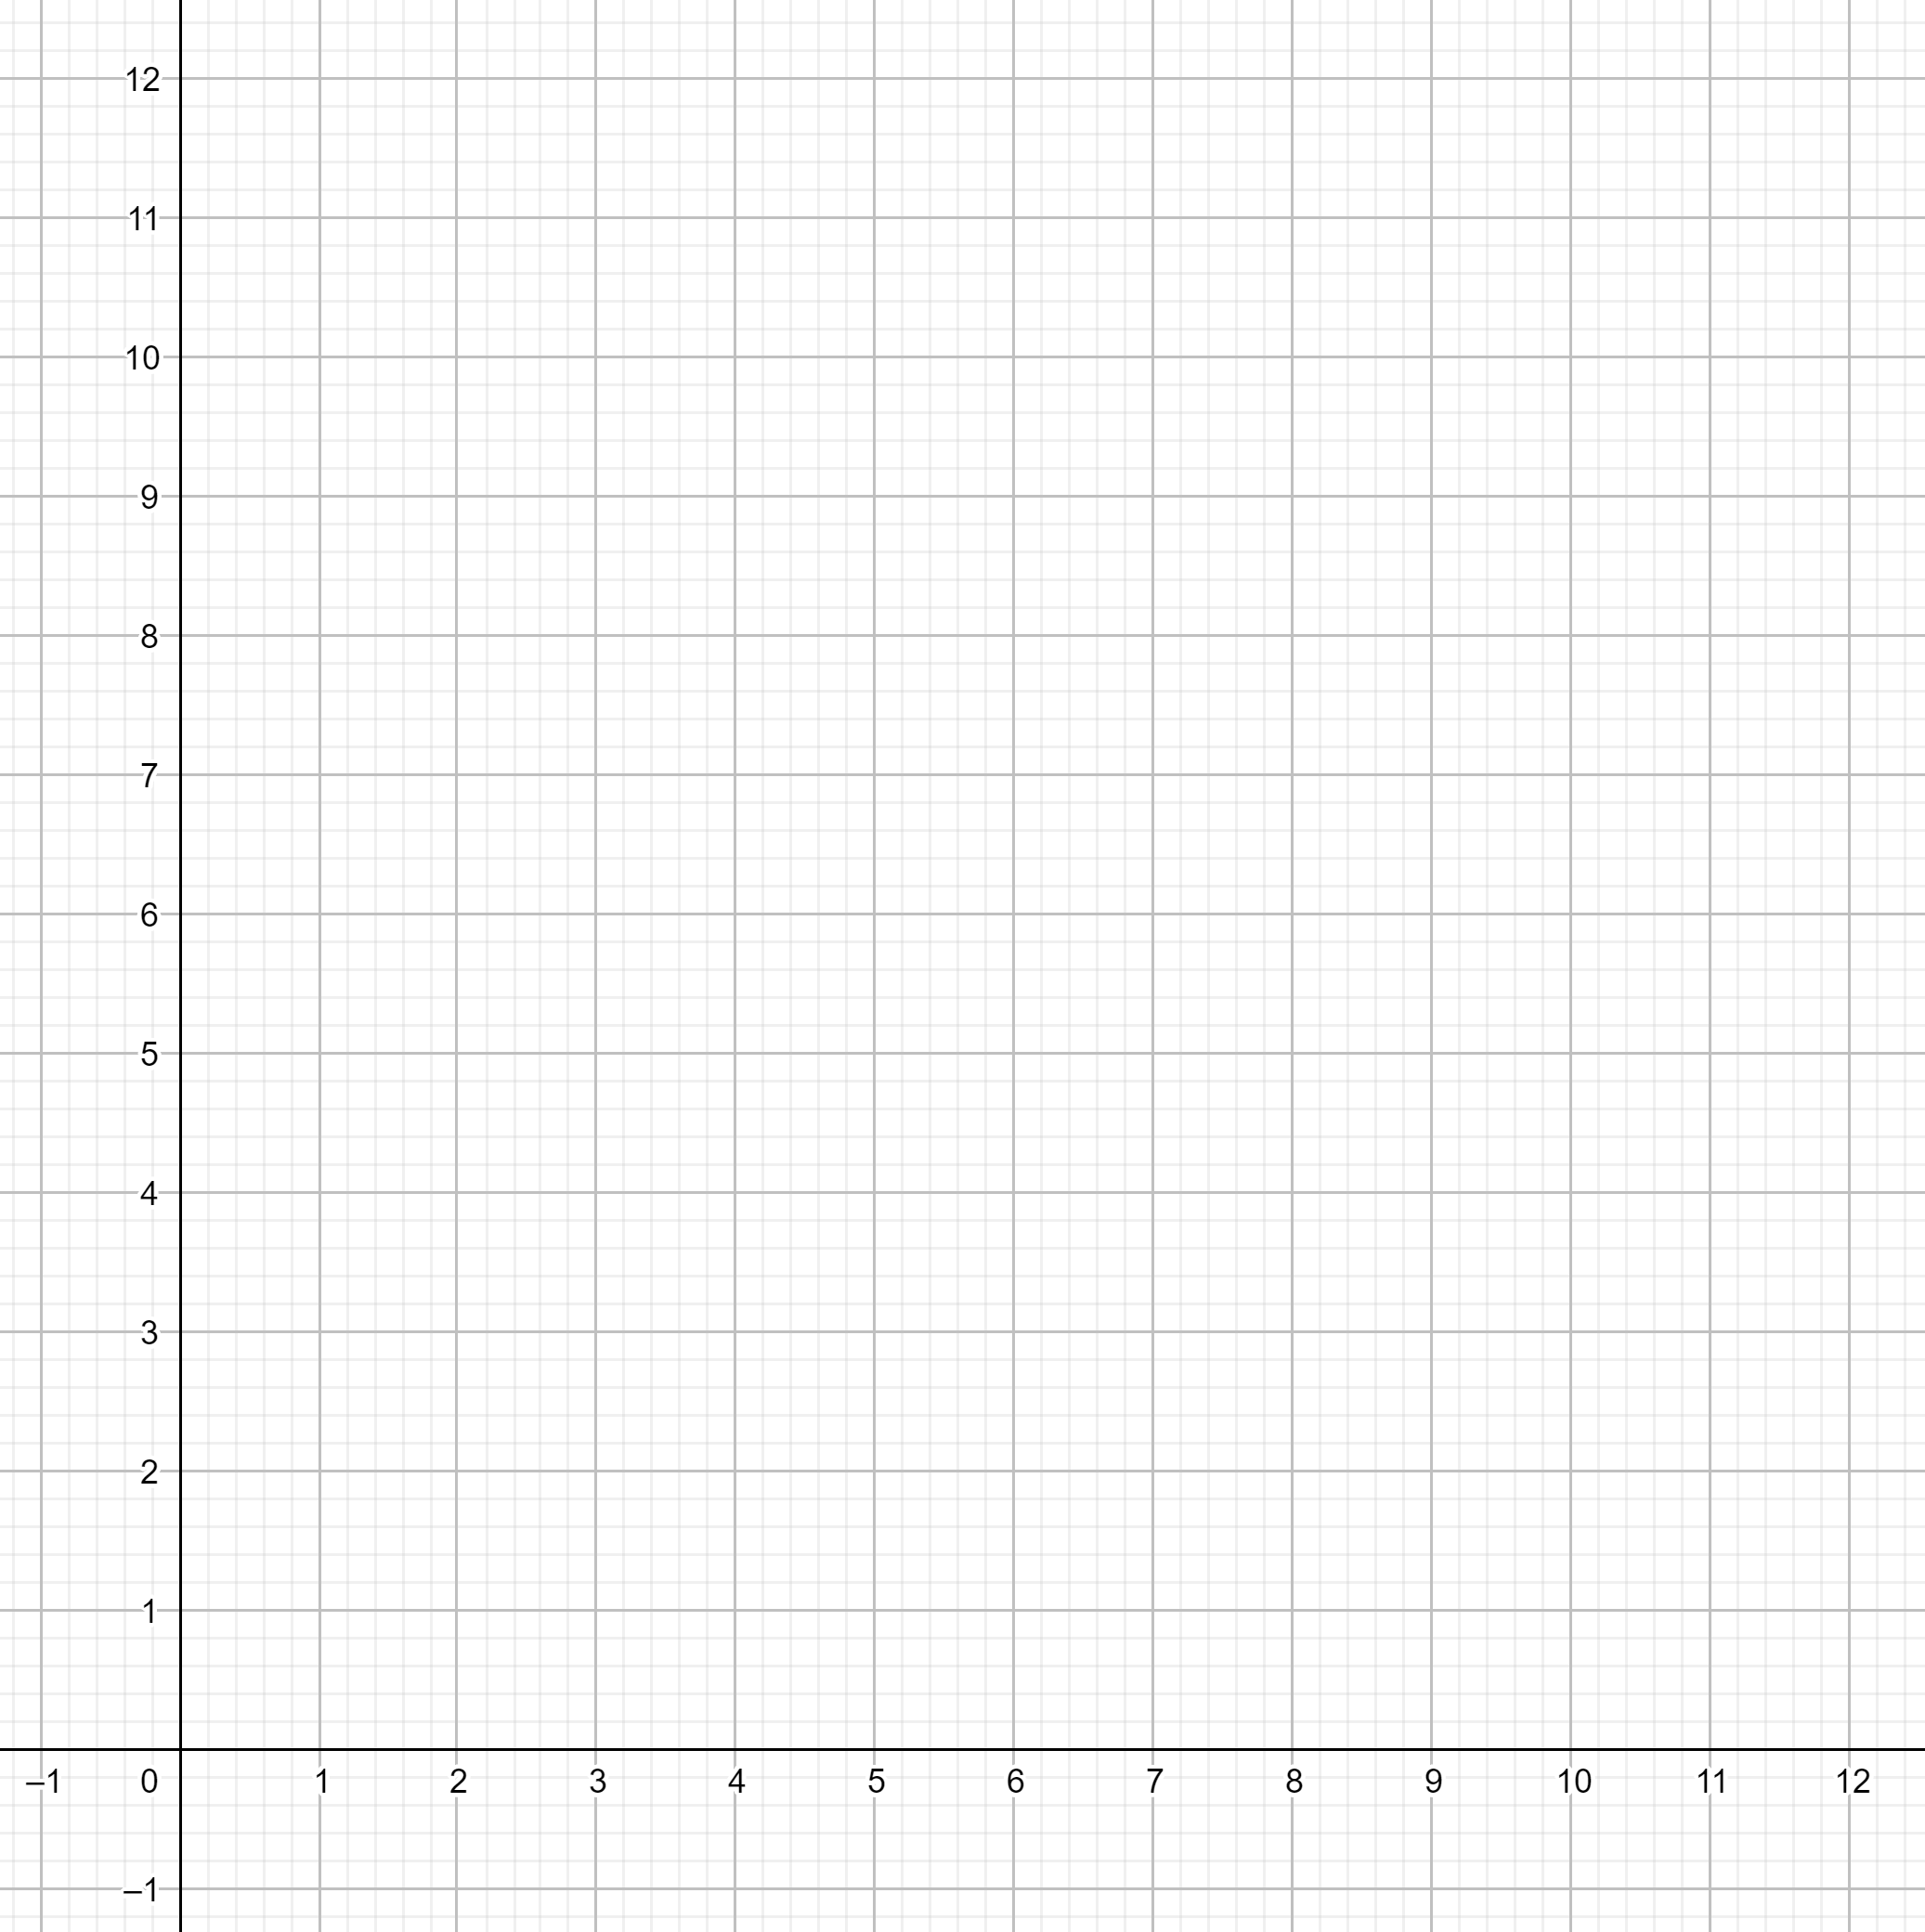
\includegraphics[scale=0.5]{vide}
\end{center}
\begin{questions}
	
	
	
	\question[2] Tracer la droite correspondant à la fonction $f(x) = -2x + 3$
	
	
	\fillwithdottedlines{3cm}
	
	\question[2]Tracer la droite d'équation $ y  = \frac{1}{2}x - 1$
%	
	\fillwithdottedlines{3cm}
	
	\question[2] Tracer la droite de coefficient directeur $a = 2$ passant par le point $B(-8; -2)$.
	

\end{questions}

\section{}

\begin{center}
	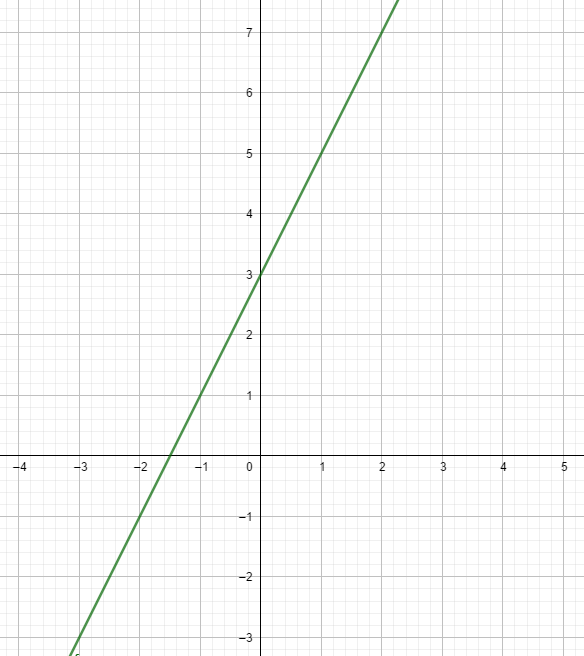
\includegraphics[scale=0.5]{fct1}
	
\end{center}

\begin{questions}
	\question[2] Déterminer la fonction représentée par la droite ci-dessus.
	\fillwithdottedlines{7cm}
	
	\question[2] Déterminer par la calcul si le point $M(2; 7)$ appartient à la droite.
	
	\fillwithdottedlines{4cm}
\end{questions}

\label{LastPage}

\newpage
\setcounter{section}{0}
\setcounter{page}{1}
\maketitle


\section{Additions}

Calculer les additions suivantes :
\begin{questions}
	
	\question[1]  $(-15) + (+ 5)$
	\fillwithdottedlines{1cm}
	\begin{solution}
		
	\end{solution}
	
	\question[1]  $(+20) + (+ 40)$
	\fillwithdottedlines{1cm}
	\begin{solution}
		
	\end{solution}
	
	
	
	
	\question[1]  $(-305) + (-27)$
	\fillwithdottedlines{1cm}
	\begin{solution}
		
	\end{solution}
	
	
	\question[1]  $(-35) + (+27)  + (-20)$
	\fillwithdottedlines{1.5cm}
	\begin{solution}
		
	\end{solution}
	
	
	\question[2]  $(-35) + (-27)  + (+20)$
	\fillwithdottedlines{1.5cm}
	\begin{solution}
		
	\end{solution}
	
	
	
	
	\question[2]  $(-75) + (-25) + (+37)$
	\fillwithdottedlines{1.5cm}
	\begin{solution}
		
	\end{solution}
	
	
	\question[2]  $(+85) + (-17) + (+15) + (-23)$ 
	\fillwithdottedlines{2cm}
	\begin{solution}
		
	\end{solution}
	
	
%	\question[2]  $(-43) + (-25) + (+57) + (+25)$ 
%	\fillwithdottedlines{2cm}
%	\begin{solution}
%		
%	\end{solution}
\end{questions}

\section{Soustractions}

Transformer les soustractions en additions avant de les calculer
\begin{questions}
	
	
	
	
	\question[2]  $(+78) - (+24)$
	\fillwithdottedlines{2cm}
	\begin{solution}
		
	\end{solution}

	
	\question[2]  $(-34) - (+57)$
	\fillwithdottedlines{2cm}
	\begin{solution}
		
	\end{solution}	

	\question[2]  $(+24) - (-32)$
	\fillwithdottedlines{2cm}
	\begin{solution}
		
	\end{solution}	
		
	\question[2]  $(-34) + (+57) - (-23) $
	\fillwithdottedlines{2cm}
	\begin{solution}
		
	\end{solution}

	\question[2]  $(-55) - (-35) - (+27) $
	\fillwithdottedlines{2cm}
	\begin{solution}
		
	\end{solution}

	
	
	
\end{questions}

\label{LastPage}
\end{document}